% 
%  $Author: awl8049 $
%  $Date: 2012/03/22 01:14:09 $
%  $Revision: 1.28 $
%
\documentclass[times, 10pt,twocolumn]{IEEEtran} 
\usepackage{amsmath,amsthm,amsfonts,amscd} % Some packages to write mathematics.
\usepackage{setspace}
\usepackage{pdfpages}
\usepackage{graphicx}
\DeclareGraphicsExtensions{.png,.jpg,.pdf,.eps}
\graphicspath{{graphics/}}
%\usepackage[caption=false,labelfont=sf,textfont=sf,captionskip=5pt]{subfig}
\usepackage{authblk}
\usepackage{afterpage}
\usepackage{comment}
\usepackage{multirow}
\usepackage[section]{placeins}
\newcommand{\equationname}{Eq.\ }
\newcommand{\equationnames}{Eq.\ }
\newcommand{\figurenames}{Figs.}
% Adjust spacing on floating elements like figures and tables.
%
\renewcommand\floatpagefraction{.9}
\renewcommand\topfraction{.9}
\renewcommand\bottomfraction{.9}
\renewcommand\textfraction{.1}   
\setcounter{totalnumber}{50}
\setcounter{topnumber}{50}
\setcounter{bottomnumber}{50}
% Add a dummy command for sub-paragraph so titlesec.sty gets happy
\newcommand{\subparagraph}{}
\usepackage[]{titlesec}
\titlespacing{\section}{0pt}{2ex}{1ex}
\titlespacing{\subsection}{0pt}{1ex}{0ex}
\titlespacing{\subsubsection}{0pt}{0.5ex}{0ex}
%
\begin{document}
\title{Thermal-Aware Scheduling and Load Balancing Using Predictive
  Energy Consumption Models in High-Performance Multicore Systems} 
\author[]{Adam  Lewis} 
\author[]{Nian-Feng Tzeng} 
\affil[]{Center for Advanced Computer Studies, University of Louisiana at
  Lafayette, Louisiana 70504\\
  \{awlewis, tzeng\}@cacs.louisiana.edu }
\maketitle
\newtheorem{defn}{Definition}
\newtheorem{thm}{Theorem}
\thispagestyle{empty}
\begin{abstract}
  Modern processors crudely manage thermal emergencies through Dynamic
  Thermal Management (DTM), where the processor monitors the die
  temperature and dynamically adjusts the processor voltage and
  frequency (DVFS) to throttle down the processor when
  necessary. However, DVFS tends to yield marked degradation in both
  application performance and system reliability. Thus, pro-active
  scheduling techniques that avoid thermal emergencies are preferable
  over reactive hardware techniques like DTM.  Based on our previously
  introduced thermal Chaotic Attractor Predictors (CAPs, which take into
  account key thermal indicators and system performance metrics for
  overall energy consumption estimation within a given power and thermal
  envelope), we have developed and evaluated an effective thread
  scheduler for multicore systems.  Besides CAPs, our scheduler makes
  use of two basic principles to minimize server energy consumption: (1)
  selecting the thread with the least probability of causing a DTM in
  the subsequent time quantum, for execution on the next available core,
  and (2) migrating execution threads on thermally overextended cores to
  other cool cores via load balancing so as to observe the thermal
  envelope.  Our developed scheduler is evaluated in practice to assess
  its potential advantage resulting from thermal-awareness by
  incorporating CAPs (for temperature prediction) and basic principles
  (for energy reduction) into the existing scheduler in the FreeBSD
  operating system.  Our implemented scheduler is run on a server with
  the Intel Xeon processor for gathering measures of interest (including
  die temperature readings and execution times) when benchmark codes
  from PARSEC and SPEC CPU2006 suites are executed.  The gathered
  results reveal that our proposed scheduler exhibits reduction in mean
  core on-die temperatures by up to 12.8$^{\circ}$C\ under PARSEC
  benchmarks (which have multithreaded workloads) and by up to 3.3$^{\circ}$C\
  under mixes of SPEC CPU2006 benchmarks for concurrent  
  execution on all four server cores, while experiencing
  only 1\% to 4\% performance degradation.
\end{abstract}

\section{Introduction}
\label{sec:Introduction}
Modern processors crudely manage thermal emergencies through Dynamic
Thermal Management (DTM), where the processor monitors the die
temperature and dynamically adjusts the processor voltage and frequency
(known as Dynamic Voltage and Frequency Scaling (DVFS))
to throttle down the processor whenever necessary. However, the use of
DVFS tends to cause significant negative impacts on application performance
and system reliability \cite{Donald2006,Bircher2008,Coskun2008d}.

This paper introduces effective scheduling for preventive thermal
management that minimizes server energy consumption by (1) 
selecting the subsequent thread with the smallest thermal impact
in the next time quantum to execute on an available core, and (2)
relocating threads run on thermally overextended cores
to other available cores for load balancing.
As opposed to prior pursuit of thermal-aware
scheduling \cite{Gomaa2004,Choi2007,Yang2008,Sarood2011} that 
aimed to bound temperatures below critical thresholds, our work considers
how to schedule high workload for die temperature management across all cores.

The current generation of operating systems treats those cores in
multicore and virtualized multi-threaded processors (like those with
Intel's HyperThreading technology) as distinct logical units, called
\textit{logical cores}, which are scheduled independently.  However,
dependency and contention exist in shared resources among those logical
cores, and hence they need to be taken into account upon their
scheduling to address performance and energy efficiency.  One approach
based on software optimization at the application level aimed to make
codes themselves more aware of existing dependencies~\cite{Khan2011}.
While effective, such an approach may not be applicable in all cases and
does not possess economies of scale.  It thus calls for the need of
intelligent, thermal-aware load balancing and scheduling within the
operating system, achievable via modeling full-system energy consumption
based on computational load for effectively predicting future energy
consumption and its associated thermal change.

To this end, we arrive at a thermal model which relates server energy
consumption to the overall thermal envelope, establishing an energy
relationship between workload and overall system thermodynamics.
According to our analysis of experimental measurements of key processor
performance counter readings and performance metrics, it is found that
the measured readings and metrics do not possess linearity and are
\textit{chaotic in nature}.  Hence, our thermal model, based on a
thermal Chaotic Attractor Predictor (tCAP), takes into account key
thermal indicators (like ambient temperatures and die temperatures) and
system performance metrics (like performance counters) for system energy
consumption estimation within a given power and thermal envelope.  This
work demonstrates that effective scheduling can result from taking
advantage of our devised tCAP when dispatching jobs to confine server
power consumption within a given power budget and thermal envelope while
avoiding detrimental impact on thread execution performance.

Dealing with all cores in a multicore system, a thermal-aware thread
scheduler is highly desirable to ensure that all of the cores in such a
system are kept equally busy, realized by migrating threads over all the
cores (no matter whether in the same processors or different ones) when
necessary for load balancing in the system.  Existing schedulers aid in
processor thermal management by dispatching workloads to cores as
tightly as possible within the same processors to expose more
opportunities for power management via shutting down unused cores.
However, computation-bound server workload fully utilizes available
system cores in most times, thereby rendering such schedulers
ineffectual.  Our Thermal-Aware Scheduler (TAS) addresses this problem
by thermally balancing system workload with as little performance
degradation as possible.  

\begin{comment}
  Need to rewrite the last sentence in the following paragraph to better
  explain Charm++
\end{comment}
Our TAS is demonstrated and evaluated by adding thermal-awareness to the
existing scheduler in the FreeBSD operating system executed on Intel
Xeon (Woodcrest) processors.  Benchmarks from SPEC CPU2006 and PARSEC
suites which represent typical application server workloads, are chosen
to evaluate our TAS.  The gathered results unveil that TAS achieves
reduction in mean core Son-die temperatures by up to 12.8$^{\circ}$C\
(from 44.8$^\circ$C down to 32.0$^\circ$C) under PARSEC benchmarks
(which have multithreaded workloads) and by up to 3.3$^{\circ}$C\ under
mixes of SPEC CPU2006 benchmarks for concurrent execution on all four
server cores, while experiencing only 1\% to 4\% performance
degradation.  Our TAS compares favorably with a recent energy-aware
scheduling technique \cite{Sarood2011}, which gets core temperature
reduction by up to 4$^\circ$C (from 63$^\circ$C down to 59$^\circ$C)
when four parallel scientific applications compatible to PARSEC
benchmarks were executed on a physical 4-core Intel Xeon 5520 processor
(similar to our testbed processor).

After an overview on pertinent background and related work is provided
in Section~\ref{sec:related}, this article introduces our proposed
thermal model in Section \ref{sec:model} and explains in Section
\ref{sec:therm-chaot-attr} how the model can be used for predictive
purposes.  Section~\ref{sec:sdesign} details the design of our TAS,
which is experimentally evaluated in Section~\ref{sec:experiment}, with
obtained evaluation results included and discussed as well.
Section~\ref{sec:conclusion} offers our conclusion.

\section{Background and Related Work}
\label{sec:related}
The thread scheduler of an OS kernel is responsible for placing threads
in the dispatch queue, deciding which threads to run next on available
logical cores, and managing thread migration to balance the workload
amongst all cores.  In addition, a scheduler must fulfill two major
applications requirements: (1) making equal progress on all threads of a
given application, and (2) exploiting as much hardware parallelism as
possible~\cite{Hofmeyr2010}. Traditional server load balancing has
various assumptions about workload behavior when making thread placement
decisions.  In particular, interactive workloads are assumed to involve
independent tasks that remain quiet for extended periods.  Server
workloads, on the other hand, are assumed to contain large numbers of
threads which are highly independent of each other and use
synchronization objects to ensure mutual exclusion on small data items.
Modern operating systems (such as Linux and Solaris) make load balancing
more power-aware by placing workloads to cores as tightly as possible
(inside fewest processors possible), thereby presenting more
opportunities for power management software to shutdown unused resources
\cite{Sun2009,Sun2009b,Xia2010}.

The following subsections provide in sequence, background and prior work
pertinent to thermal modeling, scheduling with load balancing support,
and chaotic behavior of energy consumption observed in our prior
article.

\subsection{Thermal Modeling}
\label{sec:thermal-modeling}
Existing thermal models all required to fit targeted mathematical
expressions based on time-series observations of temperatures during the
course of executing various workloads.  Expression coefficients were
estimated by minimizing total least square errors between modeling
results and actual temperature readings.  After proper calibration, such
a mathematical expression becomes a model for extrapolating future
temperatures.  Different modeling techniques have been devised.  In
particular, a model based on integer linear programming was adopted by
an earlier task scheduler~\cite{Kursun2009}, which aimed to meet
real-time deadlines while minimizing hot spots and spatial temperature
differentials across the die.  Meanwhile, dynamic thermal modeling
includes Heat-and-Run~\cite{Gomaa2004}, HybDTM~\cite{Ayoub2011} and
ThreshHot~\cite{Yang2008},\cite{Bellosa2003}.  Heat-and-Run distributes
work among available cores until the DTM events arise, and it then
migrates threads from the overheated cores to other cool cores.  On the
other hand, HybDTM enhances DTM with a thread migration strategy which
lowers the priority of jobs executed on hot cores.  Separately,
ThreshHot employs an on-line temperature estimator to determine the
proper order to schedule threads across cores, favoring those threads
which cause the greatest temperature hikes while avoiding DTM events to
occur.  Schedulers based on prior thermal modeling all rely on readings
of hardware performance counters and temperature sensors.  They can be
improved by analyzing on-die thermal variations to aid in system power
and thermal management \cite{Kursun2009}, \cite{Bailis2011}, \cite{Murali2008}.

However, preceding techniques are reactive to the temperature
approaching the DTM threshold rather than trying to avoid reaching that
temperature in the first place.  A proactive solution with multi-tier
prediction was suggested earlier \cite{Ayoub2011}, where a core level
predictor was employed to convert temperature observations to operating
frequency estimates while a control-theoretic based scheduler was
followed at the socket level for process level scheduling.  Separately,
a scheduling policy for sorting the tasks in each core's run queue
according to memory intensity was considered so as to schedule
memory-bound tasks at slower frequencies \cite{Merkel2008b,Merkel2010}.
Later, the process scheduling policy was modified in \cite{Bellosa2003}
to allocate time slices following (1) the contribution of each task to
the system power consumption and (2) the current processor temperature.
A similar approach made use of idle cycle injection to manage CPU time
slice allocation, aiming to maintain a lower average temperature over
time, as opposed to managing temperatures against a critical threshold.
Meanwhile, Cool Loop \cite{Choi2007} and Dimentrodon \cite{Bailis2011}
address a lack of heat slack by inserting additional cycles into the
task scheduling to create thermal slack, naturally leading to
performance degradation.  A variation of preceding schemes relied on
system level compiler support to insert a run-time profiling code into
applications for providing hints on the thermal intensity of a task
\cite{LiK2008}.  However, such an approach works ineffectively under
many server cases where the slack in deadlines usually is unavailable.

\subsection{Earlier Scheduling with Load Balancing Support}
\label{sec:therm-comp-workl}
Modern multiprocessor operating systems (such as Windows, Linux,
Solaris, and FreeBSD) often take a two-level approach to task scheduling
for maximized system resource utilization.  Such an approach uses a
distributed run queue and follows fair scheduling policies to manage
each core at the first level.  Its second level balances the work load
by redistributing tasks across the queues.  In particular, the FreeBSD
ULE scheduler \cite{Roberson2003,McKusick2004,McKusick2004b} uses a
combination of push and pull thread migration for load balancing.
\textit{Push migration} scans the run queues associated with each
processor every 500 milliseconds to pick the most-loaded and
least-loaded logical cores before equalizing their run-queues.  The
processor then attempts to pick a core in the same processor group so as
to minimize the migration cost.  In \textit{pull migration}, a processor
checks if it has excess work in its run queue and also if another
processor in the system is idle, before adding new thread to its run
queue.  The existence of an idle processor triggers an inter-processor
interrupt to migrate the new thread to the idle processor.  Such
two-level schedulers work under three assumptions: (1) threads are
independent, (2) load is governed by queue length, and (3) locality
exists and is important \cite{Hofmeyr2010}.  In practice, however,
common servers often have the following characteristics: (1) their
threads are logically related, with data and control dependencies among
threads, and (2) their threads have equally long life spans
\cite{Hofmeyr2010}, rendering previous two-level scheduling ineffective.

Meanwhile, existing operating systems have made their load balancing
schemes more power-aware by taking advantages of their power management
drivers which intend to find as compact an allocation of processes to
run-queues as possible \cite{Sun2009,Sun2009b,Xia2010,Sarood2011}.  This
way presents more opportunities for the power management software to
shutdown unused resources.  Such power-aware load balancing, while
effective for interactive workloads, works only if system resources are
not completely utilized; it becomes nonviable if the system workload is
high (common to high-performance servers).

\subsection{Chaotic Behavior of Energy Consumption}
\label{sec:chaot-pred-energy}
An analytical model of server energy consumption was built earlier
\cite{Lewis2008,Lewis2010} by modeling energy consumption as a
function of the work done by the system in executing its computational
tasks and of residual thermal energy given off by the system in doing
that work.  The resulting dynamic system expresses energy consumption in
the time domain as follows:
\begin{equation}
  \label{eq:system}
  E_{system}=f(E_{proc},E_{mem},E_{em},E_{board},E_{hdd})
\end{equation}
where each of the terms in the above equation is defined as: (1)
$E_{proc}$: energy consumed in the processor due to computations, (2)
$E_{mem}$: energy consumed in the DDR SDRAM chips, (3) $E_{em}$: energy
taken by the electromechanical components in the system, (4)
$E_{board}$: energy consumed by peripherals that support the operation
of the board, and (5) $E_{hdd}$: energy consumed by the hard disk drive
during the system's operation.

The continuous system in \equationnames~\eqref{eq:system} can be viewed
as a multi-variate differential equation in the time domain that can be
estimated using a time series representation. This time series is
constructed by considering (1) an initial energy state $E_{system}$ at
time $t=0$ and (2) a set of physical predictors that approximate the
values of $E_{proc}$, $E_{mem}$, $E_{board}$, and $E_{hdd}$ at the next
interval $t+\Delta t$.

% \begin{figure}[tbph]
%  \centering
%   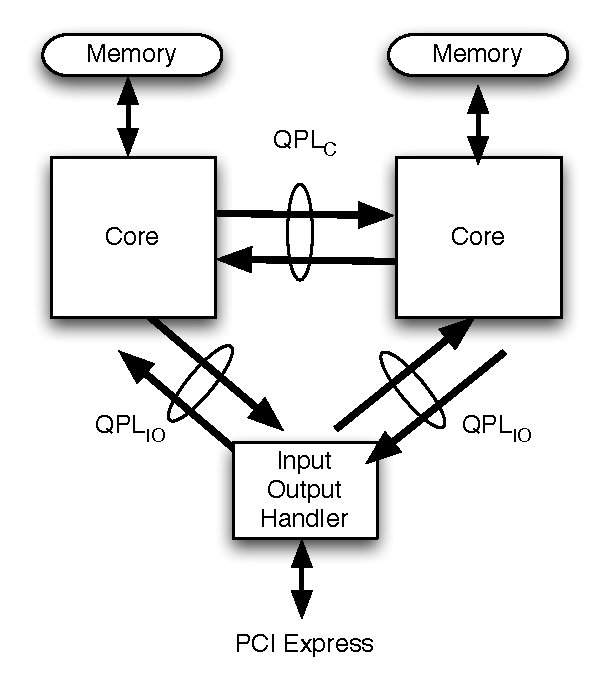
\includegraphics[scale=0.5]{intelnehalem}
%  \caption{Intel Xeon (Woodcrest) architecture.}
%   \label{fig:intarch}
% \end{figure}

\begin{table}[tbhp]
  \centering
  \caption{PeCs and performance metrics for Intel Xeon server}
  \label{tab:intelmodel}
  \begin{tabular}{l l}
\hline
\hline
\textbf{Variable}&\textbf{Measurement} (for $m$ cores and $k$ fans)\\
\hline
\hline
\multicolumn{2}{l}{\textit{Application length}}\\
$IR$&Instructions retired \\
\hline
\multicolumn{2}{l}{\textit{Application data set}}\\
$QPL_{P_{t}}$&Transactions on the QPLs between Pair $P_{t}$ of cores\\
$QPL_{IO}$&Transactions on QPLs for IO handler\\
$CM_{i}$&Last-level cache misses in Core $i$, $0\leq i$ < $m$\\
$D_{r}$&Disk bytes read\\
$D_{w}$&Disk bytes written\\
\hline
\multicolumn{2}{l}{\textit{Physical core temperature}}\\
$T_{C_{i}}$&Core $C_{i}$ on-die temperature, $0\leq i$ < $m$\\
\hline
\multicolumn{2}{l}{\textit{System temperature}}\\
$T_{A_{i}}$&Ambient temperature sensor $i$, $0\leq i$ < 3\\
\hline
\multicolumn{2}{l}{\textit{Electromechanism}}\\
$F_{j}}$&Speed of memory cooling fan $j$, $0 \leq j$ < $k$\\
\hline
  \end{tabular}
\end{table}

Observations from each time series are measured using (1)~the
appropriate PeCs for the targeted processor (2)~operating system kernel
virtual memory statistics, and (3)~processor die temperatures and
chassis ambient temperatures.  The inputs for our predictor is listed in
Table~\ref{tab:intelmodel}.  They are classified into five groups, each
associated with one server energy contributor.  As one contributor,
application length is estimated in each time period by the quantity
$IR$, the total number of retired instructions of the thread.  Among the
contributor of "application data set" listed in
Table~\ref{tab:intelmodel}, $QPL_{P_{t}}$ and $QPL_{IO}$ are relevant to
QuickPath Links, and they are associated with $E_{proc}$ and $E_{mem}$,
respectively.  Each $CM_{i}$ measures the total last-level cache miss
counts due to Core \textit{i}, $0 \leq i$ < $m$, $m$ being the number
of cores in the processor, and they determine $E_{mem}$.  As the
contributor of "physical core temperature," the core die temperature
measures are pertinent to $E_{proc}$.  The subsequent measures dictate
$E_{board}$, obtained from three temperature sensors placed on the board for
ambient temperature readings and $F_{j}$ (for $0\leq j$ < $k$) speed information measures from the $k$ memory cooling fans; those temperature readings and speed measures together determine $E_{em}$.

\subsection{Limitations of Existing Scheduling}
\label{sec:shortc-comp-workl}
Current power management software that utilizes DVFS techniques to
address DTM events has been effective in addressing thermal emergencies
\cite{Donald2006,Hanson2007}, commonly implemented in modern server
processors \cite{AMD2007,Intel2009}.  However, handling DTM through DVFS
can be problematic due to issues with program phase behavior and
contention for shared resources \cite{Bircher2008,Coskun2008d},
resulting directly from slow transitions between the active and the idle
device states and also from inability to access resources associated
with idle processors.  When the power phase changes frequently, abundant
thermal variations among cores within the processor occurs, leading to
decreased reliability \cite{Rosing2007,Coskun2008d,Kursun2009}.  For
example, the Intel XScale processor was reported to decrease its
component MTTF (Mean Time to Failure) by 12\% to 34\%, depending upon
the selected power management strategy \cite{Rosing2007}.

Work migration for energy savings and thermal management has a long
history in the SMP, SMT, and CMP environments
\cite{Yao1995,Gomaa2004,Kumar2006,Yang2008}.  A study of OS-level
thermal migration using Linux on the IBM POWER5
processor~\cite{Choi2007} discovered that the rise and fall times of
core temperatures vary in the order of hundreds of milliseconds.  As
most operating systems choose scheduler ticks to be of 10 ms or less, it
often is impossible to react to thermal conditions before a critical
state is reached.  As a result, three improvement mechanisms for
managing thermal states have been pursued: (1) core hopping for
leveraging spatial heat slack, (2) task scheduling for leveraging
temporal heat slack, and (3) SMT scheduling for leveraging temporal heat
slack.  In the presence of slack, each of those mechanisms may reduce
core die temperatures by 3 to 5$^{\circ}$ C on an average, at the
expense of 3\% mean performance degradation ~\cite{Choi2007,Ayoub2009}.
However, in the absence of slack commonly found under heavy workloads in
high-performance servers, the three mechanisms becomes ineffective,
calling for suitable scheduling with thermal awareness proactively.

\section{System Thermal Model}
\label{sec:model}
In this section, we introduce a system thermal model built upon what was
reviewed in Section \ref{sec:chaot-pred-energy} to address the thermal
domain by first considering how to extend
\equationname~\eqref{eq:system} to account for energy consumed during 
application execution.

An application is composed of $p$ execution threads, each associated with a
data set sized $d_{i}$, for $1\leq i \leq p$, in a processor. The total
data associated with $A$ is the sum of the data associated with its
component threads:
\begin{equation}
\label{eq:totaldata} D_{A}=\displaystyle\sum_{i=1}^{p}{d_i}.
\end{equation} 
We assume that the activities take place (1) in a staging area,
which contains both main and virtual memory operating space,
and (2) in the processor with its cores and their associated caches.
The execution time measurement includes 
computation time and the time to move application data from the
staging area (on peripherals off the chip like DRAM and HDD) to a
computation or operation area (on the chip, such as the caches and the cores).

Each application $A$ with the problem size of $D_{A}$ involves workload
$W(\tau_{i},d_{i},t_{i})$, for $1 \leq i \leq p$, comprising two
components: (1) a count of the operations performed by the computational
core, and (2) the count of communication operations required for
transferring data, instructions, and data coherency and book-keeping
functionality traffic.  They are measured in terms of the number of
bytes operated upon or transferred over, during the course of completing
those instructions retired by the logical core for each thread $p$.
Thus, energy consumed by executing application $A$ with data set $D_{A}$
can be expressed as:
\begin{equation}
\label{eq:eworkload} 
E_{A}(A,D_{A},t) = \displaystyle \sum_{i=1}^{p}W(\tau_{i},d_{i},t_{i})
\end{equation}
for $1\leq i \leq p$, where $\tau_{i}$ is an execution thread involved in
application $A$, $d_{i}$ is the corresponding data set for that thread,
and $t_{i}$ is its thread execution time.

In order to relate system energy expenditure (upon application
execution) to corresponding joule heating, we define the term of
``Thermal Equivalent of Application'' (TEA), as the electrical work
converted to heat in running the application, leading to die temperature
change and ambient temperature change of the system.  Hence, the TEA of
application $A$ is expressed by:
\begin{equation}
\label{eq:tea} \Theta(A, D_{A}, T, t) =
\frac{E_{A}(A, D_{A}, t)}{\displaystyle \lim_{T \to T_{th}} J_e(D_{A}, \Psi_{cp}) (T -T_{nominal})},
\end{equation} 
where $T_{th}$ denotes the threshold temperature at which a thermal
emergency event will occur, and $T_{nominal}$ refers to the nominal
temperature as reported by the system when it is in a quiescent state,
i.e., only the operating system is running without any application
execution.  The term $J_{e}$ is the ``electrical equivalent of heat''
for the chip, which reflects the \textit{informational
  entropy} of the system due to processing the data bits
during application execution and to the black body thermal properties of
the chip packaging as well as the cooling mechanisms around the chip, as
defined by the parameter $\Psi_{cp}$.  The value of $\Psi_{cp}$ is an
ambient thermal characterization parameter provided by the hardware
manufacturer to relate temperature to power for cooling
purposes~\cite{Intel2006}.  Thus, TEA is a dimensionless quantity, with
both denominator and numerator expressing work done or energy consumed
in finishing an application.

We combine these metrics into achieved performance per unit energy
consumed by the chip:
\begin{equation}
\label{eq:thermcost} C_{\theta}(A, D_{A}, T, t)=\frac{\Theta (A, D_{A}, t)}{E_{A}(A, D_{A}, t)}
\end{equation}
This normalized quantity indicates the ``cost'' of executing an
application on a given processor, with $E_{A}(A, D_{A}, t)$ obtained
from energy consumption of individual physical components (processor,
DRAM units, HDD, motherboard, and electrical/electromechanism) given by
\equationname~\eqref{eq:system}.

\subsection{Thermal Chaotic Attractor Predictors}
\label{sec:therm-chaot-attr} 
We use the measured PeCs listed in Table~\ref{tab:intelmodel} to
estimate the quantities of $\Theta(A, D_{A}, t)$ and $E_{A}(A, D_{A},
t)$ in \equationname~\eqref{eq:thermcost}.  Specifically, thread length
is estimated in each time period by the PeC measure of $IR$, namely, the
total number of instructions retired during that thread execution.  The
total data amount associated with thread execution is measured by
summing up (1) the data bytes moved across the QuickPath links on the
processor (reflected by $QPL_{C}$ and $QPL_{IO}$), (2) last-level cache
misses ($CM_{i}$, $1\leq i \leq 4$), and (3) data read from or written
to disks.  as listed under the contributor of "application data set" in
Table~\ref{tab:intelmodel}.  System temperature is measured using the
ambient temperatures reported by the system, as listed under the
contributor of "system temperature."

Following the procedure reviewed in Section~\ref{sec:chaot-pred-energy}
(and detailed in \cite{Lewis2010}), we intend to create a thermal
Chaotic Attractor Predictor (tCAP) for
\equationnames~\eqref{eq:thermcost} as an effective means for predicting
the thermal behavior during application execution.  To this end, an
analysis on the measurement data collected from our test systems is
first performed to confirm that the behavior of the time series data can
be attributed to a certain form of chaotic behavior.  It involves
evaluating system (i.e., testbed) sensitivity to initial conditions, by
calculating the Lyapunov exponents of the time series data observed
while running various benchmarks (stated in Section V.B) on the testbed.
The Lyapunov exponent quantifies the sensitivity of a system such that a
positive Lyapunov exponent indicates that the system is chaotic
\cite{Sprott2003}.  We have found a positive Lyapunov exponent when
performing this calculation on our data set, ranging from 0.019 to 0.051
on our Intel test server, as listed in Table~\ref{tab:chaotic}.
Therefore, our collected data has met the first and the most significant
criterion to qualify as a chaotic process.

The second indication of the chaotic behavior for time series
approximations expressed by \equationnames~\eqref{eq:thermcost} is an
estimate of the Hurst parameter $H$ for the time series observations. If
the value of the Hurst parameter is greater than $0.5$, an increment in
the random process is positively correlated and long range dependence
exists in the case of time series \cite{Sprott2003}.  In a chaotic
system, a value of $H$ approaching 1.0 indicates the presence of
self-similarity in the system.  As demonstrated in
Table~~\ref{tab:chaotic}, the time series data collected in our
experiments all have $H$ values close to 1.0, ranging from 0.95 to 0.99
for the Intel server in our test environment.

\begin{table}[tbhp]
\caption{Chaotic behavior in core die temperature time series}
\label{tab:chaotic} 
\centering 
\begin{tabular}{lcc}
\hline
\hline
 & Hurst exp. ($H$) & Lyaponov exp. ($\lambda$) \\
\hline
Core 0 & 0.99 & 0.051 \\
Core 1 & 0.98 & 0.019 \\
Core 2 & 0.97 & 0.034 \\
Core 3 & 0.95 & 0.040 \\
\hline
\end{tabular}
\end{table}

\section{Proposed Thermal Aware Scheduler}
\label{sec:sdesign} 
The scheduler in an operating system is responsible for making two
decisions in each time quantum: (1) thread scheduling, i.e., deciding
the next thread to run on an available core and (2) load balancing,
namely, distributing workload evenly across all cores, with existing
implementations mostly focusing on performance.  Our TAS (Thermal Aware
Scheduler) incorporates a heuristic scheduling algorithm in a popular
scheduler (i.e., ULE in the FreeBSD operating system) for thermal stress
reduction on a multicore processor while meeting the SPMD requirements
of equal execution progress and maximum parallelism exploitation.

\begin{figure}[t] \centering
  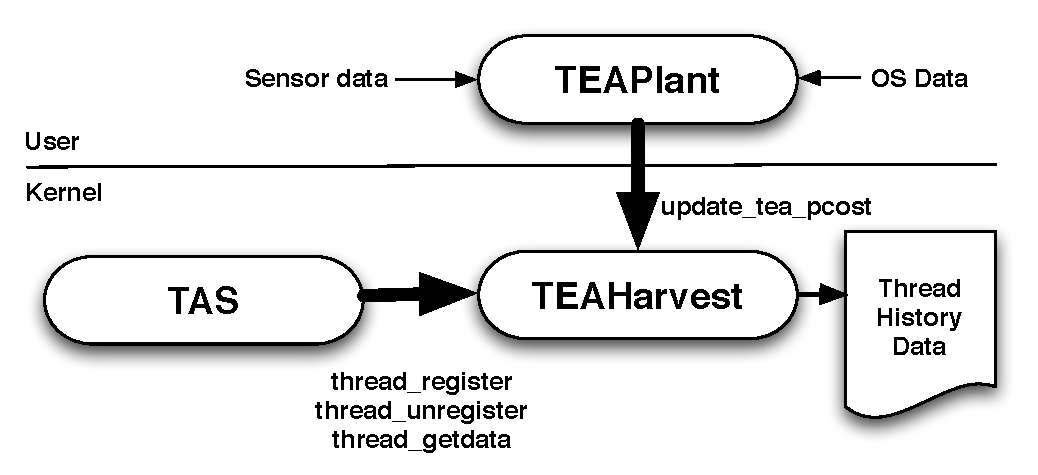
\includegraphics[scale=0.45]{tasdesign}
  \caption{TEAPlant and TEAHarvest data collection.}
  \label{fig:teaplant}
\end{figure}

\subsection{Thermal Predictors}
\label{sec:therm-pred-design} 
We enhance the existing FreeBSD operating system to maintain information
required by the thermal estimator. Our design is based on the concept of
Task Activity Vectors (TAVs) introduced earlier \cite{Merkel2008a},
with a vector for each kernel thread to store the required history in order to make
sound prediction.  Generally, the more additional space is employed
for history maintenance, the higher benefit our thermal scheduling gains.

The high-level design of TAS is shown in \figurename~\ref{fig:teaplant}.
A user-level daemon process collects required information to compute
the time-series predictions for $\Theta$ and $C_{\theta}$. Temperature
readings are collected by this process from the digital temperature
sensor associated with a core.  Similarly, processor performance
counters are gathered by the same process, with both sets of metrics
used to generate estimates. Estimates are posted via a system call
interface to a device driver that collects the data for use by
the currently executing thread.  The scheduler queries this
driver via a kernel function call interface when making scheduling
decisions to determine the $\Theta$ and $C_{\theta}$ estimates
associated with a thread.

\begin{figure}[t]
  \centering
  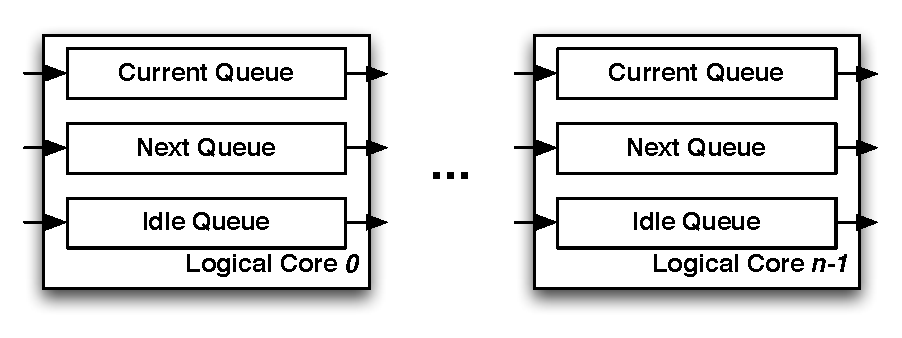
\includegraphics[height=2in,width=1.0\linewidth]{th_que}
  \caption{TAS queue structure.}
  \label{fig:tasque}
\end{figure}

\subsection{Thread Scheduling}
\label{sec:selection} 
The scheduler uses the cost predictor for $C_{\theta}$ to predict a
thread's impact on core temperature and adjust the thread priority as
required to prevent an increase in core temperature. Each core will have
one process in a running state on each scheduling interval. All other
threads will assigned by TAS to one of three queue structures maintained
per logical core: an idle queue, a current queue, and the next queue
(illustrated in \figurename~\ref{fig:tasque}).  All idle threads are
added to the idle queue and threads from this queue are executed only
the other two queues are empty.  The logical core executes all work on
the current queue in priority order and then swaps its current queue and
its next queue. For performance reasons, our implementation follows the
convention used by the existing FreeBSD ULE scheduler, placing real-time
and interrupt threads on the current queue.  This is reasonable,
given that real-time thread deadlines must be satisfied and
interrupt service routines are typically short in length.
Meanwhile, all other non-idle threads are assigned to either the current or next
queue based upon computing an interactivity score, $I$, for each thread, as follows:
\begin{equation}
\label{eq:interactsleeprun} 
I =   
\begin{cases}
  S / (SL/RUN) & \text{if sleep time} \geq \text{run time}\\
  (S/ (SL / RUN))+S & \text{if run time} < \text{sleep time}
\end{cases}
\end{equation}
where $S$ is the scaling factor of the
maximum interactivity score divided by two, and $SL$ and $RUN$ refer
respectively to the cumulative sleep and run times for the thread.
A thread with its $I$ score smaller than a predefined threshold means that
the thread had run for a very short duration during the last time window,
indicating an interactive nature of the thread (e.g., an interactive thread).   
Hence, threads whose scores fall below a predefined threshold are considered
interactive and are assigned to the current queue, with all other non-idle
threads assigned to the next queue.

For our TAS, the interactivity score $I$ is scaled by the predicted
value of $C_{\theta}$, normalized to a percentage value.  It was shown
previously \cite{Zhou2010b} that the greatest thermal benefit occurred
when a scheduler favored the thread which moved the core temperature as
close as possible to the DTM threshold without actually triggering a DTM
event.  TAS achieves a similar effect by scaling the interactivity of a
thread by its normalized execution cost, thereby giving less ``thermally
costly'' threads greater opportunities for execution so as to moderate
the processor temperature.  Penalizing more thermally costly threads
reduces the opportunities for such threads to gain access to logical
cores, presenting similar advantages of techniques which artificially
inject slack into thread scheduling but without extra scheduling
overhead incurred to those techniques.  As result, threads  with higher ``thermal
cost'' will be scheduled onto the next queue and avoid contributing to
the thermal load of the processor.   Threads on the next queue will be
scheduled to run when the queues are switched and are guaranteed to run
at least once every two queue switches, which maintains fair sharing of
the processor.

\subsection{Load Balancing}
\label{sec:loadbalance} 
Load balancing distributes workload evenly across the available logical
cores, with current implementation mostly aiming to maximize
performance.  This work applies load balancing to minimize thermal
stress while seeking best performance.  Specifically, TAS extends push
migration by organizing system cores into ``thermal clans'' based upon
the temperature and execution frequency.  Specifically, a local core is
assigned to one of the three thermal clans: Hot, Warm, and Cold, if its
on-die temperature is respectively 90\% or higher, between 75\% and
90\%, and below 75\% of the DTM threshold temperature.  Note that if a
physical core supports $\alpha$ threads, $\alpha$ logical cores will
result from the physical core, with their temperatures all equal to that
of the physical core.  In addition, logical cores are grouped into fast
and slow clans according to the execution frequencies of their
underlying physical cores.  This two-level categorization allows TAS to
manage work load distribution better from the thermal and performance
prospectives, by migrating work away from hot units with negligible
execution performance degradation.

For performance reasons, information about thermal clans of all logical
cores is maintained by the TEAHarvest thermal predictor driver.  The
driver allocates threads to local cores for execution, according to
thermal efficiency and cost estimates.  TAS scheduler queries the driver
to determine whether a core will move towards the DTM threshold
temperature if a thread becomes ready to execute on one of its logical
core.  In this way, TAS predicts whether a thread moves its assigned
core closer to a DTM event and adjusts the core's run-queue accordingly
to prevent DTM occurrence.
{\setlength{\abovecaptionskip}{0ex}
\begin{figure}[t] 
\centering
\begin{verbatim} 
 BEGIN 
   Determine if the logical core 
     is in the Hot, Warm, or Cold clan.  
   For each thread in the run queue 
     BEGIN 
       Use tCAP to estimate resulting 
         temperature change if the thread 
         is executed. 
     END 
   Determine least loaded core in the
       Cold clan.  
   Migrate the thread with worst impact 
       on temperature to logical core in
       the Cold clan most suitable from
       the speed standpoint.  
 END
\end{verbatim}
\caption{Pseudo code of TAS balancing algorithm.}
\label{fig:tascode}
\end{figure}
} 
% \begin{figure}[t] \centering
% 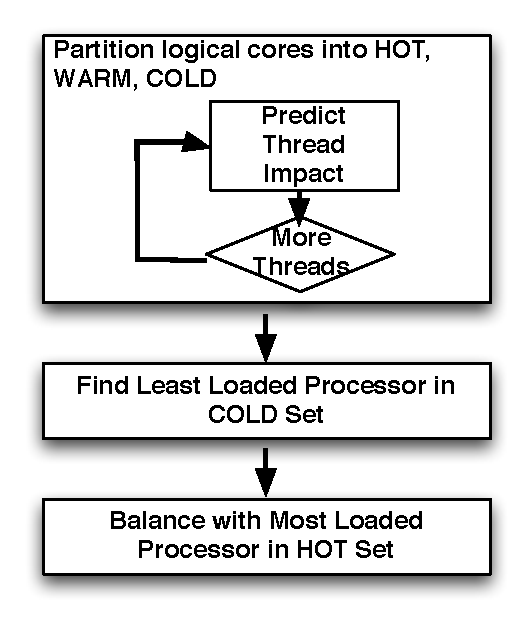
\includegraphics[scale=0.7]{tbalance.pdf}
% \caption{Design of thermal load balancing in TAS.}
% \label{fig:thermbal}
% \end{figure}
On a periodic basis (i.e., once in every 500 ms), the TAS scheduler
executes the algorithm listed in \figurename~\ref{fig:tascode} to
balance the workload among logical cores, giving sufficient times for
overtaxed resources to thermally recover.  For each thread in the run
queue, TAS uses the tCAP to estimate the value of $\Theta$ for each
thread in the queue and predict the resulting change in temperature if
this thread were to execute.  It then moves the thread with the greatest
temperature impact to the least loaded logical core in the ``Cold''
clan.  This way results in workloads being moved away from thermally
stressed logical cores, while maintaining execution performance.

\begin{figure}[t]
  \centering
  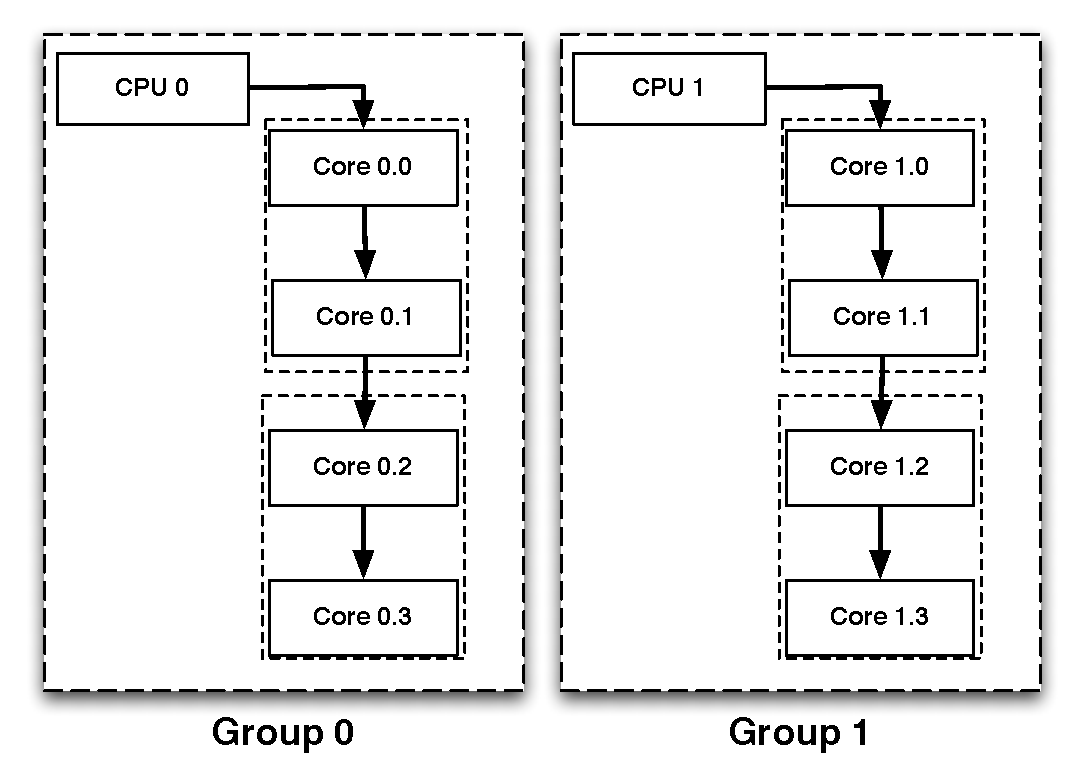
\includegraphics[width=1.0\linewidth,height=2in]{th_pgroup}
  \caption{TAS processor group example.}
  \label{fig:tasprocgroup}
\end{figure}

Execution performance is maintained by taking note of the location of
this logical core in the processor group topology.  The scheduler
inventories the processor when it starts execution and creates a
processor group structure that records the location of each logical core
n the hierarchy of physical processor sockets and physical
core~\cite{McKusick2004b}. \figurename~\ref{fig:tasprocgroup} shows the
topology generated for a dual processor configuration with four cores
per processor with pairs of cores sharing last-level cache.  The
decision of where to migrate the thread is made based upon which logical
cores in the Cold clan are located in the topology, with preference
given to logical cores that are sharing last-level caches on the same
processor.  For the example in \figurename~\ref{fig:tasprocgroup}, the
TAS would look to choose a processor from the Cold clan by selecting (1)
a thread on a logical core with whom it shares a last-level cache, (2) a
core on the same processor, and, finally (3) to a core on the other
processor.  Thus, TAS respects thread cache affinity and minimizes the
performance impact of migration of threads between logical cores.

Periodically, the system reads the temperatures of all logical cores
and, if required, also moves a logical cores to a different thermal
clan.  It should be noted that the time required for a logical core to
recover from a thermal event is significantly longer than the interval
used for thread scheduling~\cite{Choi2007}. This allows our TAS to use a
much larger interval (2 seconds) between scans (across core
temperatures) to determine if any logical core must be assigned to a new
thermal clan for better scheduling outcomes.

\section{Experimental Evaluation and Results}
\label{sec:experiment} 
We have evaluated our TAS (Thermal Aware Scheduler) using the FreeBSD
operating system run on a commodity server.  Our TAS implementation
modified the existing push migration in FreeBSD's ULE
scheduler~\cite{Roberson2003} to take into account both thermal behavior
and system performance, as elaborated in Section~\ref{sec:sdesign}.  PeC
data were collected at the user level through standard tools provided
for the data collection purpose by FreeBSD (i.e., the \texttt{coretemp}
and \texttt{hwpmc} kernel extensions).  They were collected and collated
by a FreeBSD kernel extension, made available to the operating system
scheduler for query when making scheduling decisions
(\figurename~\ref{fig:teaplant})

The processor thermal model was calibrated by measuring behavior
outcomes of the testbed with TAS at idle and under high load stress
using common utilities from the FreeBSD regression test suites and
software collections.  The CPU-related behavior of our scheduler was
then characterized using integer and floating point benchmarks from the
SPEC CPU2006~\cite{Henning2006} benchmark suite.  Benchmarks from the
Princeton Application Repository for Shared-Memory Computers (PARSEC)
suite~\cite{Bienia2008} were then evaluated on the testbed to assess TAS
in terms of key metrics of interest (i.e., die temperature and benchmark
runtime) under high parallelism in the thread level.

\begin{table}[tbhp] 
\centering
  \caption{Processor used in evaluation}
  \label{tab:hardware}
  \begin{tabular}{l l} 
\hline 
\hline
&\textbf{Dell Precision 490}\\ 
\hline 
CPU&Intel Xeon 5300 (Woodcrest)\\ 
CPU L2 cache&4MB\\ 
Memory&8GB, DDR2 667Mhz with ECC\\
Internal disk&500GB\\ 
Network&1x1000Mbps\\ 
Video&NVIDA Quadro FX3400\\ 
\hline
  \end{tabular}
\end{table}
\subsection{Experiment Setup}
\label{sec:experiment-setup} 
Experimental evaluation was conducted on our testbed running TAS, with
its hardware specified in Table~\ref{tab:hardware}.  The key metrics of
interest were gathered during the course of application execution.
Power consumed was measured by a WattsUP power meter
\cite{WattsUp2006a}, connected between the AC Main and the server
testbed.  The power meter measured the total and average wattage,
voltage, and amperage over the run of a workload.  The internal memory
of the power meter was cleared at the start of each run and the measures
collected during the runs were downloaded (after execution completion)
from the meter's internal memory into a spreadsheet.

\subsection{tCAP Establishment}
\label{sec:callibration}
Since our TAS relies on tCAP (thermal Chaotic Attractor Predictor) of
the testbed for effectively predicting its thermal behavior during
application execution, it is required first to establish tCAP using
suitable applications.  In our earlier work, a few SPEC CPU2006
benchmarks were used as training applications for deciding the
coefficients of the chaotic attractor predictor \cite{Lewis2010}.  Here,
we instead employed two applications which were expected to yield the
extreme thermal results for training execution: the idle scenario and
the most stress scenario.  An idle application referred to no
application thread ready for execution and thus the testbed runs only
the OS threads, whereas the most stress application leads to the highest
processor utilization coupled with heaviest memory activities, achieved
by launching multiple instances of the FreeBSD \texttt{cpuburn} stress
testing codes for concurrent execution, one per core with symmetric
multiple threads disabled.  The \texttt{cpuburn} stress test code
implements a single-threaded infinite loop with a sequence of integer
and floating-point operations and large blocks of memory reads and
writes to thermally stress the testbed system, driving it close to a
thermal emergency.  The use of these two extreme thermal scenarios is
preferred over employing SPEC CPU2006 benchmarks for tCAP establishment,
since any typical application execution will lies between the two
extremes, as far as the coefficients of tCAP are concerned.

These two training scenarios run for 600 seconds, with PeCs sampled at
an interval of $t=5$ seconds for establishing tCAP.  The procedure for
establishing tCAP is the same as what was described earlier
\cite{Lewis2010}, and it involved three steps. First, the training set
is constructed by consolidating the observed PeCs into a time series
using geometric means.  In the second step, the Takens Embedding
Theorem~\cite{Su2010} is applied to find delay embedding, with the
nearest neighbors algorithm then employed to identify the set of
attractors using the embedded set.  Finally, our tCAP is established by
solving the linear least squares problem resulted from fitting a
multi-variate polynomial to the attractor set.  The time complexity of
establishing tCAP equals O($n ^2$), where $n$ is the number of sampled
PeCs~\cite{Lewis2010}.  Note that the establishment of the attractor set
for tCAP is required only once for a processor type, irrespective of
applications executed on the processor.

% \begin{small}
% \begin{table}[tbph]
% \caption{SPEC benchmarks used for evaluation}
% \label{tab:benchmarks} 
% \centering
% \begin{tabular}{l c p{5cm}} 
% \hline 
% \hline
% \multicolumn{3}{l}{\textbf{Integer benchmarks}}\\
% \hline 
% hmmer &  & Search gene sequence \\
% mcf &  & Combinatorial optimization \\
% \hline 
% \hline
% \multicolumn{3}{l}{\textbf{Floating-Point benchmarks}}\\ 
% \hline 
% milc &  & Quantum Chromodynamics \\
% namd &  & Fluid Dynamics \\
% \hline
% \end{tabular} % system benchmark table
% \end{table}
% \end{small}
\subsection{SPEC Benchmark Results and Discussion}
\label{sec:microarch} 
Benchmarks from the SPEC CPU2006 suite \cite{Henning2006} were used to
evaluate the thermal behavior of CPU-bound workloads executed on our
testbed with the TAS scheduler.  The benchmarks were selected to
represent real life applications under various levels of thermal
stress. It has been shown previously \cite{Choi2007,Cher2011} that
significant core-to-core and functional unit-to-functional unit thermal
variations occur on modern processors, with the result that different
workload characteristics have strong influence on the power and thermal
behavior of the processor~\cite{Jimenez2010}.  We thus consider mixing
integer and floating-point SPEC CPU2006 benchmarks for concurrent
execution on the four cores of our testbed processor.

Three workload mixes are considered, and they span a range of cases,
including high-IPC/low-IPC, hot/cold thermal profiles \cite{Kursun2008},
and integer/floating-point combinations for better evaluating our
scheduler under diverse workload variations.  They are as follows:
Workload Mix $A$ = \{\texttt{namd}, \texttt{namd}, \texttt{hmmer},
\texttt{mcf}\}, Workload Mix $B$ = \{\texttt{milc}, \texttt{milc},
\texttt{namd}, \texttt{hmmer}\} and Workload Mix $C$ = \{\texttt{milc},
\texttt{mcf}, \texttt{mcf}, \texttt{hmmer}\}.  For example, Workload Mix
$B$ involved three copies of floating-point benchmarks (i.e.,
\texttt{milc}, \texttt{milc}, and \texttt{namd}) and one integer
benchmark, \texttt{hmmer}.  The memory intensive benchmarks (for
instance, the \texttt{milc} benchmark) tend to consume more power when
executed as opposed to other benchmarks in the suite while benchmarks
with higher IPC (the \texttt{mcf} and \texttt{hmmer} benchmarks) tends
to increase core on-die temperatures.

\begin{table}[tbp] 
\centering
\caption{Temperature and runtime results under benchmark mixes}
\label{tab:mixwkload}
\begin{tabular}{cllllll} 
\hline
\hline
Workload & \multicolumn{4}{c}{Core die temperature reduction} & Runtime\\
 Mix & Core 0 & Core 1 & Core 2  & Core 3 & increase \\
\hline
$A$ & 2.8$^{\circ}$C & 1.0$^{\circ}$C & 1.7$^{\circ}$C & 2.0$^{\circ}$C & 2.1\% \\
$B$ & 1.0$^{\circ}$C & 0.8$^{\circ}$C & 2.0$^{\circ}$C & 1.1$^{\circ}$C & 2.9\% \\
$C$ & 3.1$^{\circ}$C & 3.3$^{\circ}$C & 3.0$^{\circ}$C & 2.9$^{\circ}$C & 2.5\% \\
\hline
\end{tabular}
\end{table}

It was observed that as execution progressed, the threads of those
benchmarks again tended to pin themselves to particular cores, depending
upon cache and memory utilization of other concurrent threads.  Core
temperatures are reduced under TAS in comparison to those under ULE,
with the reduction amounts listed in Table~\ref{tab:mixwkload} for the
three workload mixes.  Under Workload Mix $C$, for example, TAS lowers
core temperatures by at least 2.9$^{\circ}$C and by as much as
3.3$^{\circ}$C.  The benchmark run times (which reflect performance
degradation) increase negligibly always, ranging from 2.1\% to 2.9\%.

Involving both thermal-aware scheduling and load balancing, TAS compares
favorably with earlier workload migration-oriented methods, with
comparable reductions in average core die temperatures and performance
impact for similar workloads and processors.  Specifically,
Variation-Aware Core Hopping~\cite{Kursun2009} examined both thread
migration, by using off-line profiling of processor thermal variation to
guide assignment of threads to cores, and thread selection, by using the
profiling information to guide scheduling decisions in an enhanced Linux
scheduler.  This technique was demonstrated to lower core temperatures
ranging from 2.0$^{\circ}$C to 5.5$^{\circ}$C with pairs of SPEC CPU2006
benchmarks executed an IBM POWER5 processor with minimal overhead in the
decision process. However, their implementation did not performance
impact of logical cores sharing resources and the related
migration costs entailed by not considering cache affinity in scheduling
decisions.  Meanwhile, Predict-and-Act~\cite{Ayoub2011}
employs a hybrid reactive/proactive migration policy that controls
system fan speeds while scheduling threads at the core level.  This
hybrid method  was shown
to reduce on-die core temperatures by 3$^{\circ}$C to 4$^{\circ}$C on a
"simulated" pair of quad-core Intel Xeon processors (rather than a real
implementation) when executing mixes of SPEC2006 benchmarks similar to
those in our study.

\begin{table}[tbp] 
\centering
 \caption{PARSEC benchmarks used in evaluation}
\label{tab:parsecbench}
\begin{tabular}[bthp]{l l p{5cm}} 
\hline 
\hline 
bodytrack &  & Computer vision image tracking application \\
canneal &  & Simulated annealing chip routing cost computation \\
facesim &  & Physical simulation of facial behavior \\
ferret &  & Content-based similarity search \\
freqmine &  & Simulate FP-growth method for Frequent Itemset Mining \\
streamcluster &  & Online clustering algorithm for data mining \\
swaptions &  & Simulated pricing of portfolio options \\
\hline
\end{tabular}
\end{table}
\subsection{PARSEC Benchmark Results and Discussion}
\label{sec:mult-behav} 
Selected benchmarks from the PARSEC~\cite{Bienia2008} suite, described
in Table~\ref{tab:parsecbench}, were used to evaluate our TAS as well.
They were compiled with the POSIX \texttt{pthreads} library and executed
using the PARSEC \texttt{native} input sets.  Being parallel workloads
selected from the fields of computer vision, computational finance,
enterprise servers, and animation physics (see Table~\ref{tab:parsecbench}), PARSEC
benchmarks better represent real life applications than SPEC CPU2006 and
can benefit markedly from scheduling their abundant independent threads
freely based on thermal prediction.

\begin{figure}[tbp] 
\centering
  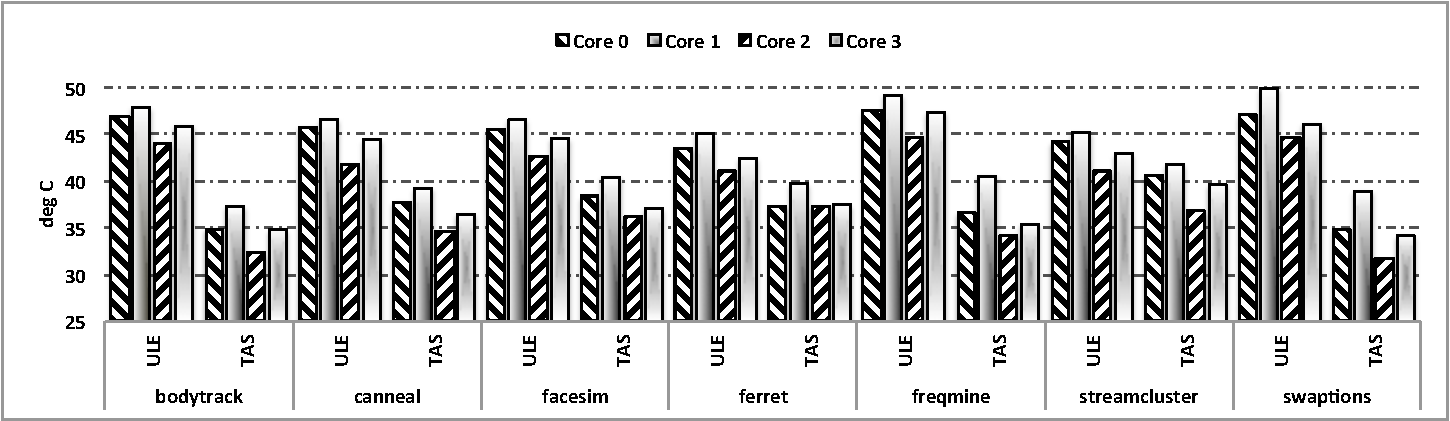
\includegraphics[width=1.0\linewidth,height=1.7in]{graphics/parsectemp}
  \caption{Comparison of PARSEC benchmark average core die temperatures
under ULE and TAS schedulers.}
  \label{fig:pbenchmarkt}
\end{figure}
Three behavior metrics of interest under TAS are gathered: (1) the
average core on-die temperature, (2) the benchmark run time, and (3)
mean system power dissipation.  The outcomes of average core on-die
temperatures upon executing those seven PARSEC benchmarks are depicted
in \figurename~\ref{fig:pbenchmarkt}.  As can be seen from the figure,
the core on-die temperatures range from 32$^\circ$C (for Benchmark
\texttt{swaption}) to 42$^\circ$C (for Benchmark \texttt{streamcluster})
under TAS, with \texttt{swaption} and \texttt{bodytrack} (or
\texttt{streamcluster}) experiencing the lowest (or highest) mean
temperature across the four cores.  Temperature outcomes for the same
benchmarks under the classical ULE scheduler are also included in
\figurename~\ref{fig:pbenchmarkt} for comparison.  It is found that
temperature reduction amounts are larger for benchmarks with smaller
working sets (like \texttt{bodytrack} and \texttt{swaptions}).  This is
because such a benchmark has a lower cache requirement \cite{Bienia2011}
and thereby lets TAS schedule threads more freely according to thermal
prediction with negligible performance degradation, resulting in better
temperature reduction.  Consequently, TAS enjoys temperature reduction
by more than 12.8$^{\circ}$C (from 44.8$^{\circ}$C down to
32.2$^{\circ}$C) for the \texttt{swaptions} benchmark.
  
Benchmarks with streaming functions, such as \texttt{facesim},
\texttt{freqmine}, and \texttt{streamcluster}, all have large working
sets, which hinder TAS from scheduling threads freely based on thermal
prediction, since doing so degrades performance considerably.  Hence,
those benchmarks tend to yield less temperature reduction under TAS,
with the average core on-die temperature lowered by 3-6$^{\circ}$C.  

Execution performance (measured in terms of the benchmark runtime) under TAS 
is depicted in \figurename~\ref{fig:pbenchmarkp}.
When compared with the runtime results under ULE included in the figure,
it can be observed that TAS leads to negligible performance degradation,
by no more than 3.3\% for all benchmarks examined except \texttt{streamcluster}.
Considerable performance degradation is seen for Benchmark \texttt{streamcluster},
however, likely due to its high computational intensity as the data set
grows with rising dimensionality and thereby calling for
more synchronization required.
As a result, TAS experiences noticeable performance degradation
when scheduling threads based on thermal prediction.

\begin{figure}[tbp]
  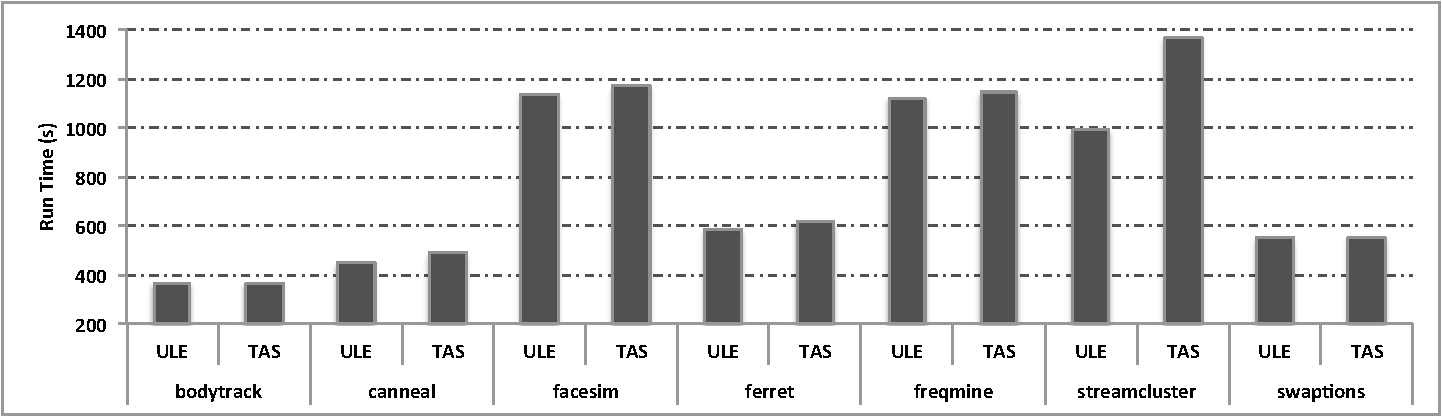
\includegraphics[width=1.0\linewidth,height=1.3in]{graphics/parsecperformance}
  \caption{Comparison of PARSEC benchmark performance under ULE and TAS
schedulers.}
  \label{fig:pbenchmarkp}
\end{figure} 
\begin{figure}[tbp]
  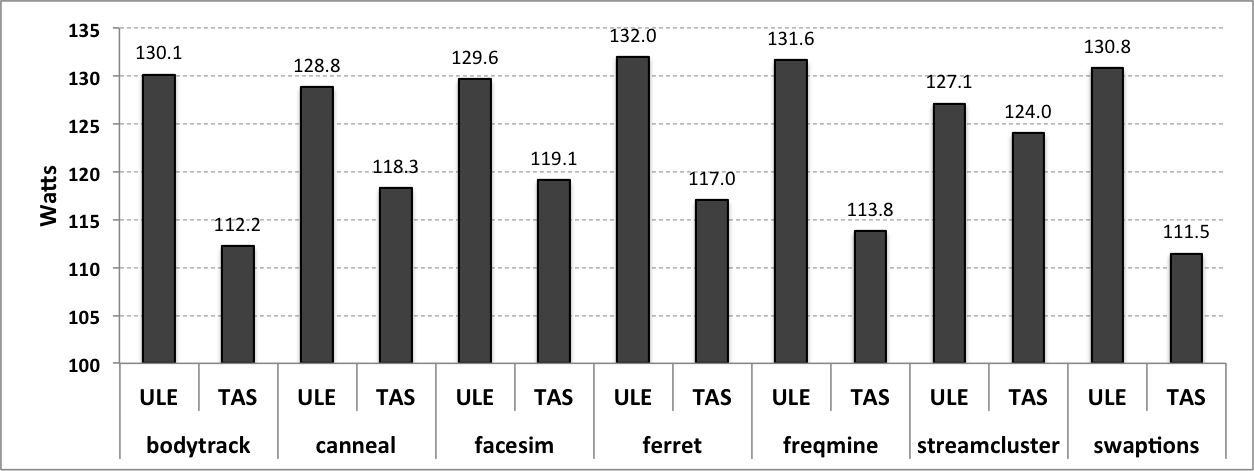
\includegraphics[width=1.0\linewidth,height=1.3in]{ParsecPowerConsumption.png}
  \caption{Comparison of PARSEC benchmark average power dissipation under ULE and TAS schedulers.}
  \label{fig:pbenchmark}
\end{figure}
\begin{figure}[tbp]
  \centering
  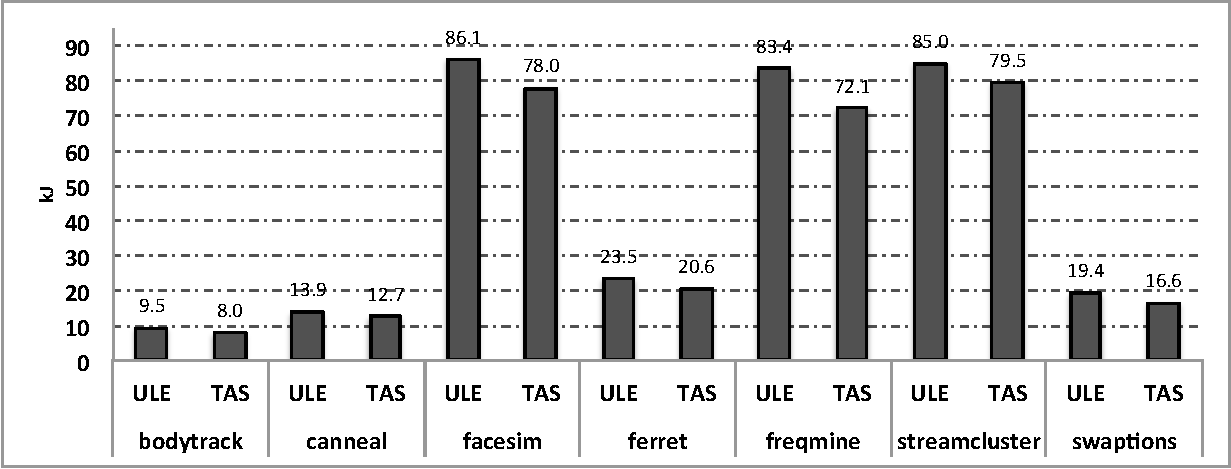
\includegraphics[width=1.0\linewidth,height=1.3in]{parseckj}
  \caption{Comparson of PARSEC total energy consumption under ULE and TAS schedulers.}
  \label{fig:penergy}
\end{figure}
Mean system power dissipation for each of the PARSEC benchmarks run on our testbed
under both schedulers is shown in \figurename~\ref{fig:pbenchmark}.
When compared with ULE, TAS is observed to reduce 
power dissipation markedly, from 14W (for the \texttt{ferret} benchmark) 
to 19W (for \texttt{swaptions}), due to their relatively small working sets.
On the other hand, less reduction in power dissipation is found for
benchmarks with large working sets, lowering power by the range of
3W (for \texttt{streamcluster}) to 10W (for \texttt{facesim}).   The
total energy consumption for each of the PARSEC benchmarks run on our
testbed is shown in \figurename~\ref{fig:penergy}.   In comparison with
ULE, TAS is observed to reduce energy consumption between 2.8kJ (for
\texttt{ferret}) to 2.9kJ (for \texttt{swaptions}) for benchmarks with
relatively small working sets, resulting in 14\% to 17\% reduction.

% In \figurename~\ref{fig:tasvsedp}, we contrast the optimization strategy
% used by TAS versus other possible optimizations schemes for managing the
% trade-off between performance and energy.  In this figure, we compare
% the energy savings from TAS for \texttt{facesim} benchmark to schemes
% that minimize delay under peak power constraints (DPC) and minimize
% energy under peak power and delay constraints (EPDC). DPC minimizes the
% delay of an execution interval so that the maximum power within an
% execution interval never exceeds a limit while EPDC schemes seek to
% minimize energy while operating a system within a power budget with a
% limit on the workload performance impact.  For the TAS results, we have
% integrated the mean power dissaption over time to compute energy use to
% compute percentage energy savings and compare against results reported
% in prior work~\cite{Cochran2011}. In this case, the optimizations used
% by TAS outperforms both DPC and EPDC for the \texttt{facesim} benchmark
% by 4\% to 6\% (against reported results in prior work of mean system
% power dissipation of 108W to 115W on a quad-core Intel processor).

% \begin{figure}[bpt]
%   \centering
% 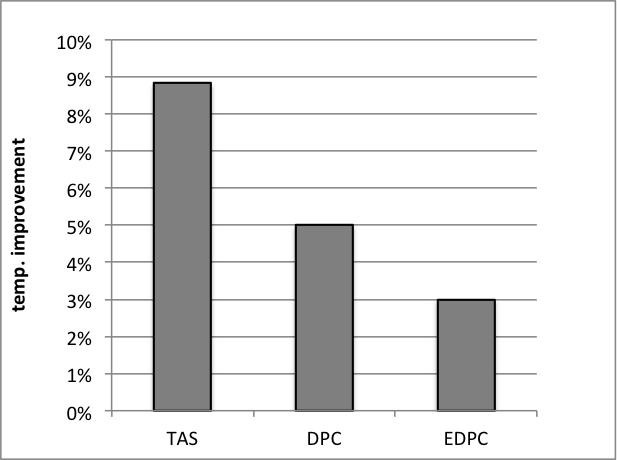
\includegraphics[width=1.0\linewidth,height=1.3in]{graphics/tasvsedpc}
%   \caption{Average percentage reduction in core die temperature for the
%     \texttt{facesim} benchmark under various optimization strategies.}
%   \label{fig:tasvsedp}
% \end{figure}
% \begin{comment}
%   Last sentence should be revised and extended per last sentence in
%   introduction. 
% \end{comment}

\section{Conclusion}
\label{sec:conclusion}
Dense servers pose power and thermal challenges, which often cannot be
addressed satisfactorily by conventional DVFS and DTM mechanisms,
especially under heavy workloads common for high-performance systems.
We have investigated into thermal-aware scheduling to deal with such
challenges, capable of managing system energy consumption within a given
power and thread envelope effectively.  As opposed to prior work aiming
to bound temperatures below critical thresholds, our proposed scheduler
considers how to dispatch heavy workloads in the high-performance
multi-core system for die temperature management across all cores.  It
is based on the thermal Chaotic Attractor Predictors (tCAPs) we develop
to guide thread selection and load balancing, taking into account key
thermal indicators and system performance metrics for preventing DTM
instances proactively.  The proposed tCAP-oriented scheduling (dubbed
the TAS scheduler) has been implemented to replace the original
scheduler of the FreeBSD operating system (called the ULE scheduler) for
evaluation on a testbed server under benchmarks from the SPEC CPU2006
and PARSEC suites.  Experimental results demonstrate that our TAS
scheduler can lower the mean on-die core temperature by up to
12.8$^{\circ}$C  
under PARSEC benchmarks and by up to 3.3$^{\circ}$C under
mixes of SPEC benchmarks for concurrent execution, while exhibiting
negligible performance degradation, in comparison to the ULE scheduler.
When compared with a recent energy-aware scheduling technique reported
to attain core temperature reduction by up to 4$^\circ$C 
(from 63$^\circ$C down to 59$^\circ$C) upon executing 
four parallel scientific applications compatible to PARSEC benchmarks 
on an Intel Xeon 5520 4-core processor \cite{Sarood2011}, our TAS
clearly enjoys better thermal reduction under multi-threaded execution.

\label{sec:references}
\bibliographystyle{ULieeetran}
\bibliography{../overall.bib}
\end{document}
% The following comment block is used by the different flavors of EMACS and
% the AUCTEX package to manage multiple documents.  In order for AUCTEX
% to understand you're working with multiple files, you should define
% the TeX-master variable as a file local variable that identifies your
% master document.
%
% Please do not remove.
%%% Local Variables: 
%%% mode: latex
%%% TeX-master: "scheduler.tex"
%%% TeX-PDF-mode: t
%%% TeX-source-correlate-mode: t
%%% End: 
